% --------------------------------------------------------------------- METHOD
\section{Data and method}
\label{sec:method}

\subsection{The motivating corpus}
\label{sec:method-corpus}

The corpus is a crawl of a large research organisation's public websites, collected for this
project between 21 March and 11 October 2022 across 80 hosts~\cite{dlrcrawl2022}. It is not a published
dataset: it is not redistributable and cannot be obtained by a reader. That is a
real limitation on reproducibility, and it is why Section~\ref{sec:neutrality} provides an
indirect check using three corpora that anyone can download.
\measured{} The raw crawl spans 45 detected languages, but English and German account for
89.7\% of it, and only those two are carried forward. The corpus's role here is to supply
realistic scale and realistic mess; the method is not specialised to it.

\begin{samepage}
\measured{} The original crawl contains 733{,}210 archived records. After language selection
and text cleaning, the final corpus used for production labelling contains 616{,}499 records:
423{,}966 English and 192{,}533 German. Each record represents an archived capture of a page.
Distinct records can therefore share the same URL or contain identical text.
\end{samepage}

\begin{table}[h]\centering
\caption{Number of records in the original crawl and the final corpus used for production
labelling.}
\label{tab:corpus}
\begin{tabular}{lr}
\toprule
Stage & Records \\
\midrule
Original crawl                  & 733{,}210 \\
Final English--German corpus    & \gd{616{,}499} \\
\bottomrule
\end{tabular}
\end{table}

Production labelling uses the final 616{,}499-record corpus. Some earlier topic-model results
were retained without rerunning them after duplicate embedding rows were removed, as documented
in Section~\ref{sec:failures}.

\begin{figure}[t]\centering
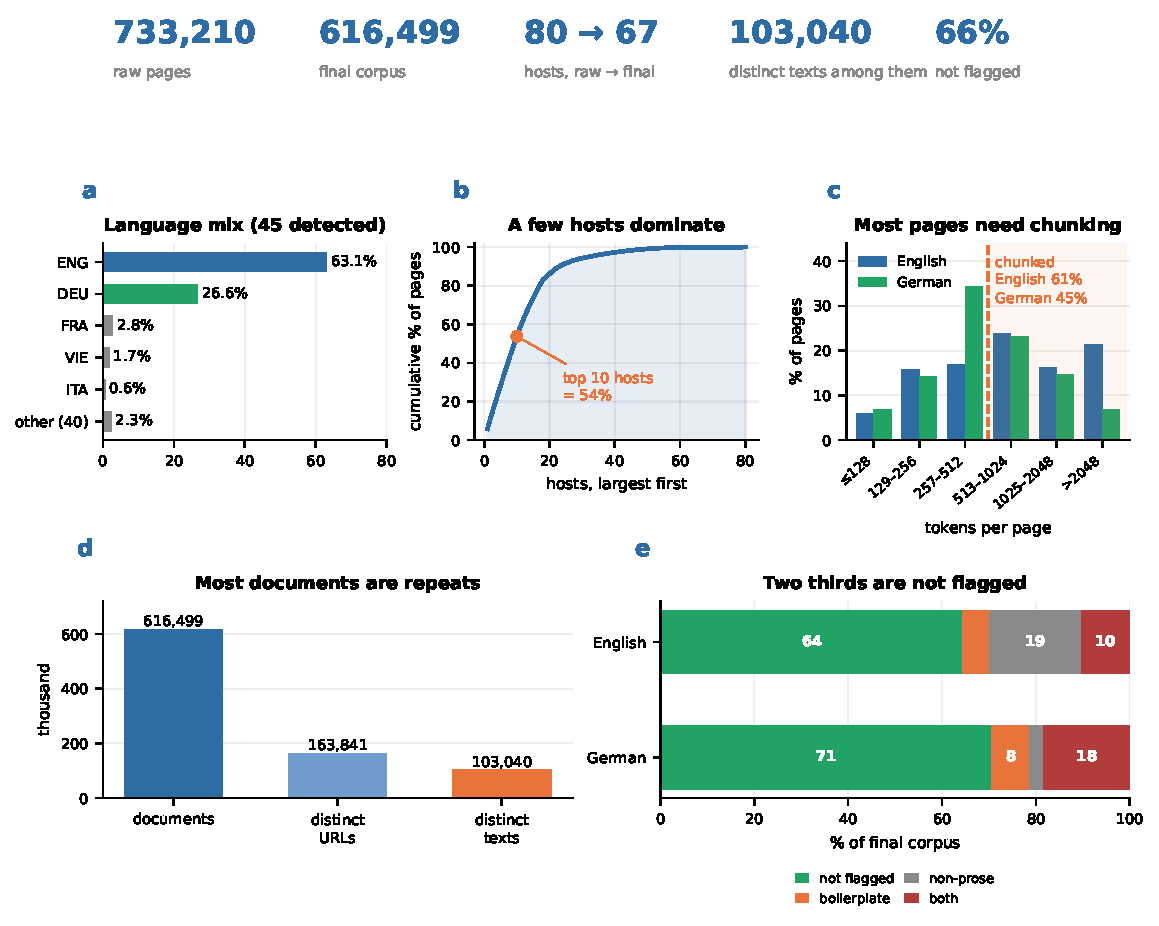
\includegraphics[width=\textwidth]{figs/fig_crawl_dashboard}
\caption{Profile of the DLR crawl. The strip gives the headline counts.
\textbf{(a)}~Detected languages in the raw crawl; records without a detected language are not
shown. Only English and German are modelled.
\textbf{(b)}~Cumulative share of pages held by the largest hosts, where a host is a subdomain of
\texttt{dlr.de}.
\textbf{(c)}~Share of pages in the final corpus in each length band, in tokens, against the 512-token
window of the embedding model; pages right of the dashed line must be split into chunks.
\textbf{(d)}~The 616{,}499 documents in the final corpus correspond to only 163{,}841 distinct URLs and
103{,}040 distinct texts, because the same page was fetched repeatedly.
\textbf{(e)}~Share of pages in the final corpus by the pipeline's boilerplate and non-prose flags.}
\label{fig:dashboard}
\end{figure}

\measured{} Figure~\ref{fig:dashboard} profiles the crawl. In the raw crawl English is 63.1\% of pages (462{,}595) and German 26.6\%
(195{,}133). A further 54{,}309 pages are in 43 other detected languages, and 21{,}173 have no
detected language. Among the other detected languages, French is the largest at 2.8\% of the raw
crawl, followed by Vietnamese at 1.7\% (Figure~\ref{fig:dashboard}a). Ten hosts hold 53.7\% of the raw
crawl and the largest alone 5.9\%, so the corpus is dominated by a few large sites
(Figure~\ref{fig:dashboard}b).

Two properties of the data drive design decisions later on. First, the same page is fetched
repeatedly: the final corpus holds 616{,}499 documents but only 163{,}841 distinct URLs
(3.8 per address) and only 103{,}040 distinct texts (6.0 documents per text;
Figure~\ref{fig:dashboard}d). The duplicate-removal step removes repeated copies of the same
record. Different captures with the same URL or text remain, so user-facing results must also
be de-duplicated by normalised address. Second, \measured{} the pipeline's detectors flag 33.6\%
of pages in the final corpus as boilerplate, non-prose or both. These flags target material such
as navigation, staff directories, search interfaces, privacy notices and machine-generated
artefacts. The flags were not checked page by page (Figure~\ref{fig:dashboard}e).

\subsection{The control and benchmark corpora}
\label{sec:method-benchmarks}

The crawl has no labels, so correctness cannot be measured on it directly. Four additional
corpora are used: one control for RQ1 and three labelled benchmarks for an indirect test of RQ3.
Topic models are fitted separately on each corpus. The corpora are deliberately unlike the crawl,
because transfer to dissimilar data is what the data-neutrality constraint of Section~\ref{sec:intro-neutrality}
requires in practice. Table~\ref{tab:datasets} lists them and Figure~\ref{fig:benchdash}
profiles them.

\begin{table}[h]\centering
\caption{The corpora used. Class shares are those of the largest and smallest class; the
largest is also the purity obtained by assigning every document to one cluster
(Section~\ref{sec:neutrality}). The control corpus carries no class labels in this work.}
\label{tab:datasets}
\small
\begin{tabular}{llrrrrr}
\toprule
Corpus & Language & Documents & Classes & Largest & Smallest & Median words \\
\midrule
DLR crawl (this work)~\cite{dlrcrawl2022}
                        & EN, DE & 616{,}499 & none & --- & --- & 310 \\
GDELT Ahrtal (control)~\cite{leetaru2013gdelt}
                        & DE     & 3{,}873 & none & --- & --- & 710 \\
\addlinespace
20 Newsgroups~\cite{lang1995newsweeder}
                        & EN     & 17{,}792 & 20 & 5.4\%  & 3.3\% & 89 \\
Reuters-21578~\cite{lewis1997reuters}
                        & EN     & 7{,}980  & 10 & 48.9\% & 1.4\% & 72 \\
10kGNAD~\cite{block2019gnad}
                        & DE     & 10{,}265 & 9  & 16.3\% & 5.2\% & 298 \\
\bottomrule
\end{tabular}
\end{table}

\begin{figure}[t]\centering
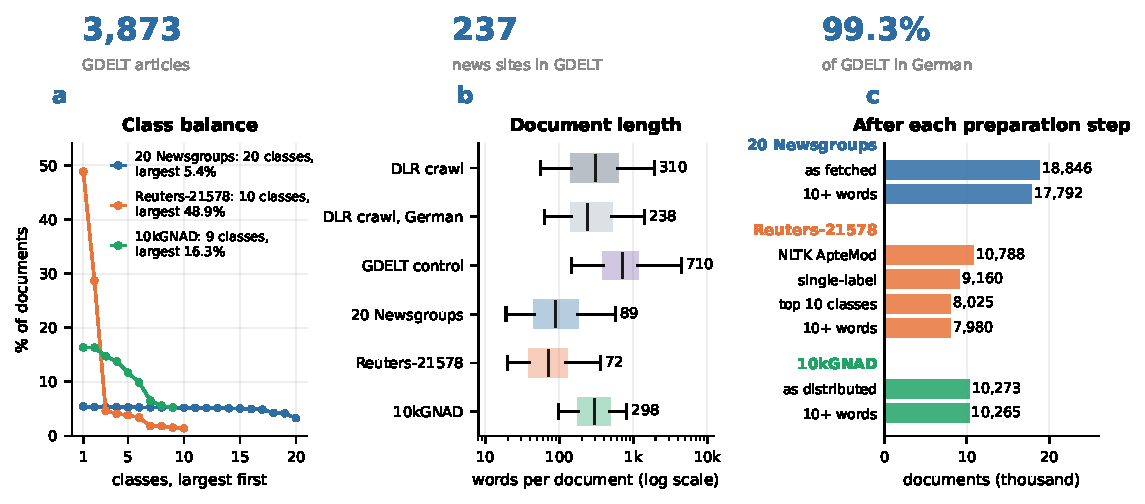
\includegraphics[width=\textwidth]{figs/fig_benchmark_dashboard}
\caption{Profile of the control and benchmark corpora. The strip gives the headline counts.
\textbf{(a)}~Share of documents in each class, largest class first, for the three labelled
benchmarks.
\textbf{(b)}~Words per document. Each box spans the middle half of the documents, the whiskers
the 5th to 95th percentile, and the number is the median.
\textbf{(c)}~Documents left after each preparation step.}
\label{fig:benchdash}
\end{figure}

\begin{samepage}
\paragraph{Preparation.} Documents under ten words are dropped from all three benchmarks.

20 Newsgroups has its headers, footers and quoted text removed, the
standard step that stops a model learning email boilerplate in place of
topics~\cite{sklearn20ng}. After this preparation and the minimum-length filter, 17{,}792 of
18{,}846 documents remain.
\end{samepage}

Reuters-21578 is taken from the ApteMod version distributed with NLTK (10{,}788 documents).
Only documents with one label are kept. Of these, only the ten most frequent categories are
retained, giving 8{,}025 documents. The minimum-length filter leaves 7{,}980.

10kGNAD, derived from the \emph{Der Standard} articles of the One Million Posts
corpus~\cite{schabus2017million}, is used as distributed. The minimum-length filter reduces
it from 10{,}273 to 10{,}265 documents (Figure~\ref{fig:benchdash}c).

\paragraph{Why these three.} 20 Newsgroups and Reuters-21578 are both English-only, which would
leave the German half of the pipeline with no external check, although German is a third of the
corpus (31.2\%). 10kGNAD was added to close that gap; its median length (298 words) is close to
the German crawl's (238). 20 Newsgroups has classes of nearly equal size, whereas almost half of
Reuters is one class (Figure~\ref{fig:benchdash}a). This matters when interpreting purity; Section~\ref{sec:experimental-purity-floor}
explains its lower bound.

\paragraph{The control corpus.} The GDELT control is a collection of 3{,}873 news articles about
a single event, the July 2021 flood in the Ahr valley, selected through GDELT's Global Knowledge
Graph~\cite{leetaru2013gdelt}. The articles come from 237 news sites and have GDELT-recorded dates
between July 2021 and August 2024, more than half of them in July 2021; 99.3\% are in German. It carries
no class labels. We use this corpus to check whether the difficulty comes from the
topic-discovery methods, the noisy DLR crawl, or both. GDELT covers the flood and the response
to it, so we expect a small number of topics. If a method still selects many topics here, this
points to a limitation of the method. If it selects only a few on GDELT but many on DLR, this
suggests that the DLR data explains the difference (Section~\ref{sec:rq1-nok}).

\measured{} The silhouette sweep in Figure~\ref{fig:gdelt-silhouette} supports this expectation. It tests different group counts
and compares how closely documents group together and how separate the groups are. On the
3{,}842 prepared articles, its highest score is 0.798 at $K=2$, meaning two groups, among the
tested values $K=2,4,\ldots,40$.\footnote{\raggedright The sweep uses Ward clustering on vectors
reduced to 50 coordinates with UMAP, scored by cosine silhouette. Saved configuration and
scores: \texttt{output/gdelt\_ahrtal/}\allowbreak\texttt{discover\_k/}, files
\texttt{k\_config.json} and \texttt{discover\_k\_silhouette.json}.}

\noindent\begin{minipage}{\linewidth}
\centering
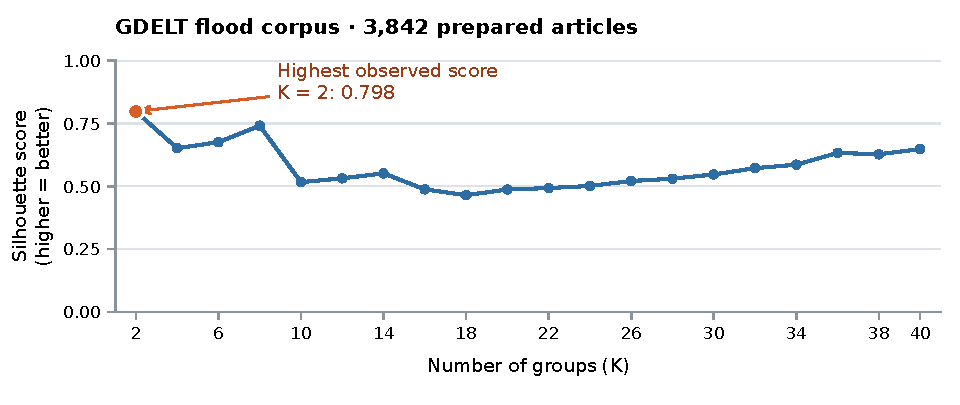
\includegraphics[width=\linewidth]{figs/fig_gdelt_silhouette.pdf}
\captionof{figure}{Silhouette sweep on the GDELT control. \measured{} Each dot is a tested
group count; lines connect the saved scores. The highlighted maximum occurs at the smallest
tested count. The prepared articles and scoring method are described above.}
\label{fig:gdelt-silhouette}
\end{minipage}

\paragraph{What the statistics drive.} \measured{} In the final corpus, the median page is 310
words and a quarter are under 148. The 5th to 95th percentile runs from 55 to 1{,}934 words, and
3.8\% of pages are under 50 words (Figure~\ref{fig:benchdash}b). Pages that short are hard to place.

Long pages raise a different problem. After text cleaning, 52.9\% of pages require more than one
chunk: 57.2\% in English and 43.4\% in German. Each chunk accommodates 494 text tokens, as
explained in Section~\ref{sec:method-embed}.

For comparison, a sample of 60{,}000 pages from the raw crawl has a median of 299 words, with
10\% of pages under 50 words. The final corpus contains a smaller share of very short pages.
This comparison combines language selection, minimum-length filtering and text cleaning.

The benchmark comparison has a separate implication. The two English benchmarks are far shorter
than the crawl, while 10kGNAD has a similar median length (Table~\ref{tab:datasets} and
Figure~\ref{fig:benchdash}b). These curated discussion and news collections differ from a
heterogeneous website crawl. They therefore provide a limited test of how the method handles
navigation pages, directories and other page types (Section~\ref{sec:limitations}).

\subsection{Pipeline}
\label{sec:method-pipeline}

The pipeline uses each page's cleaned body text as input. RQ2 (Section~\ref{sec:rq2}) explains
why body text was chosen.

Figure~\ref{fig:pipeline} summarises the production pipeline. The following subsections explain
embedding, topic discovery and document labeling in that order. The separate analyses used to
answer RQ3 are described in Section~\ref{sec:rq3}.

% ---------------------------------------------------------- PIPELINE FIGURE
\begin{figure}[!tb]
\centering
\begin{tikzpicture}[
  box/.style   = {rounded corners=6pt, draw, line width=0.9pt, minimum width=9.0cm,
                  minimum height=1.30cm, align=center, inner sep=7pt},
  flow/.style  = {-{Stealth[length=3mm,width=2.4mm]}, line width=1.1pt, draw=black!72},
  feed/.style  = {-{Stealth[length=2.6mm,width=2.1mm]}, line width=0.8pt, dashed,
                  dash pattern=on 3.2pt off 2.6pt},
]

% ---- nodes -----------------------------------------------------------------
\node[box, fill=black, draw=black, text=white] (data) at (0,0)
  {{\large\bfseries DLR webpage data}\\[1pt]
   {\footnotesize\color{black!25} Web pages $\cdot$ German $+$ English $\cdot$ no labels}};

\node[box, fill=fillblue, draw=boxblue, below=0.80cm of data] (embed)
  {{\footnotesize\scshape\color{boxblue} Embedding}\\[2pt]
   {\large\bfseries E5 --- body text as embeddings}\\[1pt]
   {\footnotesize multilingual-E5-large-instruct, 1024-dim}};

\node[box, fill=fillgreen, draw=boxgreen, below=0.80cm of embed] (cluster)
  {{\footnotesize\scshape\color{boxgreen} Clustering}\\[2pt]
   {\large\bfseries BERTopic}\\[1pt]
   {\footnotesize topics from a filtered sample, c-TF-IDF keywords}};

\node[box, fill=fillred, draw=boxred, below=0.80cm of cluster] (label)
  {{\large\bfseries Labelling}\\[1pt]
   {\footnotesize\color{boxred} nearest centroid, all documents}};

% ---- main flow -------------------------------------------------------------
\draw[flow] (data)    -- (embed);
\draw[flow] (embed)   -- node[right, font=\footnotesize, text=boxgreen] {sample} (cluster);
\draw[flow] (cluster) -- (label);

% ---- side feed: cleaned body text bypasses the embedder ------------------
\coordinate (lrail) at ($(data.west)+(-1.30,0)$);
\draw[feed, draw=diagray] (data.west) -- (lrail) |- (cluster.west);
\node[rotate=90, font=\footnotesize\color{diagray}, anchor=south]
  at ($(lrail)!0.5!(lrail|-cluster.west)+(-0.12,0)$) {cleaned body text};

% ---- side feed: E5 vectors reused for assignment ---------------------------
\coordinate (rrail) at ($(embed.east)+(1.30,0)$);
\draw[feed, draw=boxblue] (embed.east) -- (rrail) |- (label.east);
\node[rotate=-90, font=\footnotesize\color{boxblue}, anchor=south]
  at ($(rrail)!0.5!(rrail|-label.east)+(0.12,0)$) {all E5 vectors};

\end{tikzpicture}
\caption{The core document-assignment pipeline. E5 embeds all documents; BERTopic learns topics
from a filtered sample per language. The dashed paths supply cleaned body text for keywords
and all E5 vectors for nearest-centroid assignment. Every document receives a topic, including
those outside the sample.}
\label{fig:pipeline}
\end{figure}


\subsection{Document embeddings with E5}
\label{sec:method-embed}

The embedding model is \texttt{intfloat/}\allowbreak\texttt{multilingual-e5-large-instruct}
\cite{wang2024multilingual}. It converts each document's cleaned body text into a vector: a
list of 1{,}024 numbers representing the text. English and German use the same model. A fixed
task instruction asks it to identify the page's main research topic. The resulting vectors are
reused for topic discovery and document labeling.

E5 accepts 512 tokens, where a token is a word or part of a word. \measured{} In the
text before cleaning, the median page uses 1.84 tokens per word, so the window holds roughly 280
words; 56.1\% of pages are longer (Figure~\ref{fig:dashboard}c);
cutting those at 512 tokens would discard on average 54.8\% of their text. An attempt to raise the
window to 1{,}024 tokens failed because the model does not support that input length.

The fix adopted instead is to split each document into chunks that fit the window, embed
each chunk, and average the resulting vectors. Each chunk must also hold the model's 16-token task
instruction and two special tokens, which leaves 494 tokens of text, and the production embedding run keeps
at most eight chunks per document: its first 3{,}952 tokens.

Figure~\ref{fig:embedding-chunks} shows how pages are split into chunks and how much text the
eight-chunk limit leaves unread.
\measured{} On pages with text beyond this limit, an average of 51.4\% of their cleaned text
is left unread.
Most pages are read in full; the longest are represented by their beginning.

\noindent\begin{minipage}{\linewidth}
\centering
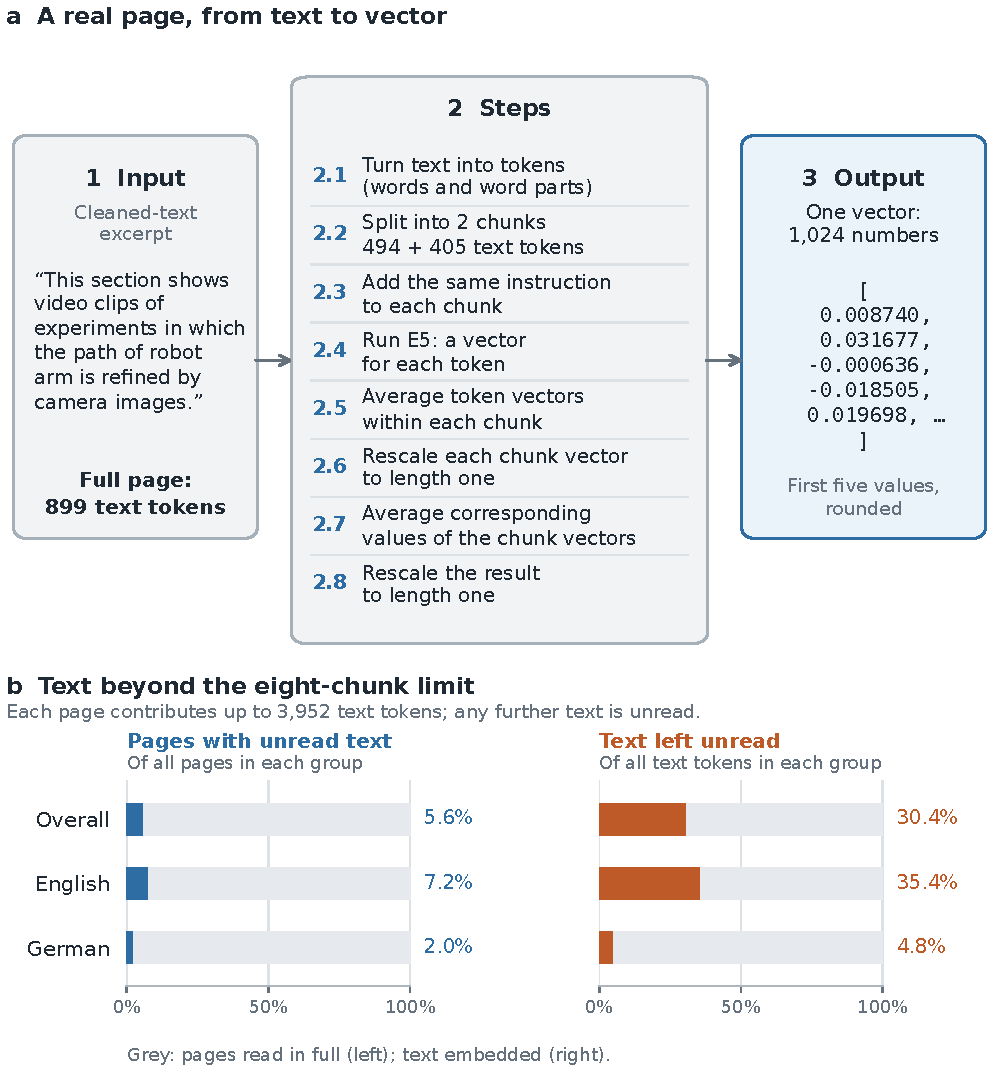
\includegraphics[width=\linewidth]{figs/fig_embedding_chunks.pdf}
\captionof{figure}{Chunking with E5. (a) \measured{} A real example using the robotics page
``Video Clips'' (saved crawl entry \texttt{eee5510b-60c1-4f6d-80e4-6a5f06cd3b2f}). The input is
an excerpt; the vector represents the full page. Only its first five values are shown, rounded
for display. The numbered steps separate tokenisation, E5 encoding and averaging. Rescaling
applies the same multiplier to every value in a vector.
(b) \measured{} Blue shows the percentage of pages with text beyond the limit. Orange shows
the percentage of all cleaned-text tokens beyond the limit. Overall, 5.6\% of pages have unread
text; their unread portions amount to 30.4\% of all text tokens because these pages are very
long. Each language row uses its own pages and text tokens.}
\label{fig:embedding-chunks}
\end{minipage}

E5 was chosen in part because it was trained to use task instructions, or prompts~\cite{wang2024multilingual}.
The aim was to guide the model towards research content and uncover topic structure hidden
in noisy web text.
% Exploratory evidence: output/stage2_lang/{eng,deu}/eval_results.json and
% output/stage2_lang_persona/{eng,deu}/eval_results.json.
\measured{} The limited prompt comparison in Section~\ref{sec:setaside-persona} did not
establish a consistent benefit from changing the instruction. Further prompt development was
not pursued because of time limits and because it was not needed to answer the three research
questions.

\subsection{Topic discovery with BERTopic}
\label{sec:method-bertopic}

Topic discovery runs separately for English and German on a sample of each language. Before
sampling, URL filters exclude page types such as code listings and catalogue pages from the
pool used to discover topics. These filters limit which documents shape discovery; the later
labeling step still covers the full corpus. The earlier model and language comparisons are
reported in Section~\ref{sec:setaside-models}.

BERTopic~\cite{grootendorst2022bertopic} receives the existing E5 vectors. UMAP
\cite{mcinnes2018umap} first reduces the number of coordinates used to represent each vector.
HDBSCAN~\cite{campello2013hdbscan} then finds dense groups: documents close together in that
reduced space. Documents that do not join a group receive the noise label $-1$.
The production setting uses \texttt{min\_topic\_size=100}, which sets the minimum cluster size;
the number of topics is not fixed in advance. Section~\ref{sec:rq3} examines that setting.

The groups receive descriptive keywords from their documents' cleaned body text. BERTopic
uses class-based TF-IDF, which scores words within each topic relative to the other topics.
The vectors determine the groups; the text supplies their descriptions. These discovered
topics are the input to document labeling. Figure~\ref{fig:bertopic-pipeline} shows these steps.

% Discovery flow in scripts/run_bertopic.py. Existing vectors are reused;
% cleaned text supplies the c-TF-IDF descriptions. The input example reuses the
% verified saved page and vector from Figure 5; the flow describes the full sample.
\noindent\begin{minipage}{\linewidth}
\centering
\begin{tikzpicture}[
  stage/.style = {rounded corners=4pt, draw, line width=0.8pt,
                  text width=2.50cm, minimum height=2.30cm,
                  align=center, inner xsep=4pt, inner ysep=5pt,
                  font=\small\sffamily},
  flow/.style = {-{Stealth[length=2.2mm,width=1.7mm]},
                 line width=0.9pt, draw=black!65},
  side/.style = {flow, dashed},
]

\node[font=\small\sffamily\bfseries, text=accent, align=center,
      text width=6.2cm] at (3.2,3.65)
  {Run separately for\\English and German};

\node[stage, minimum height=4.50cm, fill=fillblue, draw=boxblue] (input) at (0,0)
  {\textbf{1 Input}\\[4pt]
   Saved E5 vectors\\
   One real example:\\[5pt]
   {\footnotesize\ttfamily
    [\\
    0.008740,\\
    0.031677,\\
    -0.000636,\\
    -0.018505,\\
    0.019698,\\
    \ldots ]}};

\node[stage, fill=fillgreen, draw=boxgreen] (reduce) at (3.2,0)
  {\textbf{2 UMAP}\\[4pt]
   Reduce the\\number of\\coordinates};

\node[stage, fill=fillgreen, draw=boxgreen] (cluster) at (6.4,0)
  {\textbf{3 HDBSCAN}\\[4pt]
   Find dense\\groups of\\nearby vectors};

\node[stage, fill=black!3, draw=diagray] (words) at (9.6,0)
  {\textbf{4 Keywords}\\[4pt]
   Count words\\by topic; rank\\with c-TF-IDF};

\node[stage, minimum height=4.50cm, fill=fillblue, draw=boxblue] (output) at (12.8,0)
  {\textbf{5 Output}\\[4pt]
   {\footnotesize\textbf{Shown page}\\[3pt]
    \ttfamily
    uuid: ...3b2f\\
    topic\_id: -1\\
    topic\_weights:\\
    0.0}\\[6pt]
   {\footnotesize\textbf{Another topic: 85}\\[3pt]
    robot, path,\\
    control, \ldots}};

\draw[flow] (input.east) -- (reduce.west);
\draw[flow] (reduce.east) -- (cluster.west);
\draw[flow] (cluster.east) -- (words.west);
\draw[flow] (words.east) -- (output.west);

\node[stage, text width=4.70cm, minimum width=5.10cm,
      minimum height=2.60cm, fill=black!3, draw=diagray,
      align=left, font=\footnotesize\sffamily] (text) at (9.6,4.10)
  {\textbf{Cleaned body text}\\[4pt]
   Example from the same page:\\[3pt]
   \textit{This section shows video clips of experiments in which the path of robot arm
   is refined by camera images.}};
\draw[side, draw=diagray] (text.south) -- (words.north);

\node[stage, text width=7.20cm, minimum height=1.15cm,
      fill=fillred, draw=boxred] (noise) at (6.4,-2.55)
  {\textbf{Noise label $-1$}\\[3pt]
   Keep these pages for labeling (Section~\ref{sec:method-coverage})};
\draw[side, draw=boxred] (cluster.south) -- (noise.north);

\end{tikzpicture}
\captionof{figure}{BERTopic discovery on one language sample. \measured{} The input examples
reuse the robotics page from Figure~\ref{fig:embedding-chunks}: its saved vector and a
cleaned-text excerpt. Only the first five vector values are shown, rounded; the vector
represents the full page. All sampled pages are processed together. The displayed page
received $-1$ during discovery and continues to document labeling
(Section~\ref{sec:method-coverage}). Its output row comes from \texttt{doc\_topics.parquet},
with the page ID shortened here. The separate keyword example for topic 85 comes from
\texttt{topic\_top\_words.json} and describes other sampled pages.}
\label{fig:bertopic-pipeline}
\end{minipage}


\clearpage
\subsection{Document labeling}
\label{sec:method-coverage}

\begin{enumerate}[leftmargin=*,itemsep=0.4em]
\item \textbf{Calculate centroids.} Leave out $-1$ and sample pages flagged as code or data
dumps when forming the averages. For each topic with remaining sample pages, rescale its
vectors to length one, average them, then rescale the average to length one. This is the
topic's centroid, or centre.
\item \textbf{Calculate similarity scores.} Rescale each page vector to length one, then
compare it with every available centroid for its language using cosine similarity.
This score compares vector directions; a higher value means a closer match.
\item \textbf{Assign a topic.} Give each page the topic with the highest score. If scores tie,
choose the smallest topic ID.
\item \textbf{Save the label and flags.} Store the page ID, chosen topic, score, and the flags
for repeated website text and code/data pages.
\end{enumerate}

Figure~\ref{fig:labeling-pipeline} shows these steps with real input and output examples.

% Horizontal labeling flow, matching the discovery figure's style.
% Real example values are checked against the saved sample and production files.
\noindent\begin{minipage}{\linewidth}
\centering
\begin{tikzpicture}[
  stage/.style = {rounded corners=4pt, draw, line width=0.8pt,
                  text width=2.50cm, minimum height=2.30cm,
                  align=center, inner xsep=4pt, inner ysep=5pt,
                  font=\small\sffamily},
  flow/.style = {-{Stealth[length=2.2mm,width=1.7mm]},
                 line width=0.9pt, draw=black!65},
  side/.style = {flow, dashed},
]

\node[font=\footnotesize\sffamily\bfseries, text=accent, align=center,
      text width=2.6cm] at (0,3.45)
  {Use the topics\\for the page's\\own language};

\node[stage, minimum height=4.50cm, fill=fillblue, draw=boxblue] (input) at (0,0)
  {\textbf{1 Input}\\[4pt]
   Saved E5 vectors\\
   One real example:\\[5pt]
   {\footnotesize\ttfamily
    [\\
    0.008740,\\
    0.031677,\\
    -0.000636,\\
    -0.018505,\\
    0.019698,\\
    \ldots ]}};

\node[stage, fill=fillgreen, draw=boxgreen] (average) at (3.2,0)
  {\textbf{2 Average}\\[4pt]
   {\footnotesize\textbf{Sample only}\\[3pt]
    Rescale vectors;\\
    average by topic;\\
    rescale again.}};

\node[stage, fill=fillgreen, draw=boxgreen] (compare) at (6.4,0)
  {\textbf{3 Compare}\\[4pt]
   {\footnotesize Every page against\\
    every topic vector.\\
    Pick highest score.}};

\node[stage, fill=black!3, draw=diagray] (flags) at (9.6,0)
  {\textbf{4 Flags}\\[4pt]
   {\footnotesize Mark repeated\\
    website text and\\
    code/data pages.}};

\node[stage, minimum height=6.00cm, fill=fillblue, draw=boxblue] (output) at (12.8,0)
  {\textbf{5 Output}\\[4pt]
   {\scriptsize\ttfamily
    uuid: ...3b2f\\
    label: "85"\\
    similarity:\\
    0.982268\\
    is\_boilerplate:\\
    false\\
    is\_non\_prose:\\
    false}\\[6pt]
   {\footnotesize\textbf{Topic 85 words}\\[3pt]
    robot, path,\\
    control, \ldots}};

\draw[flow] (input.east) -- (average.west);
\draw[flow] (average.east) -- (compare.west);
\draw[flow] (compare.east) -- (flags.west);
\draw[flow] (flags.east) -- (output.west);

\node[stage, text width=9.30cm, minimum width=9.70cm,
      minimum height=2.20cm, fill=black!3, draw=diagray,
      align=left, font=\footnotesize\sffamily] (metadata) at (6.4,4.50)
  {\textbf{Sample topic IDs from Section~\ref{sec:method-bertopic}, plus saved page and topic flags}\\[4pt]
   For topic averages, leave out $-1$ and pages flagged as code or data dumps.\\[3pt]
   Keep available topic vectors flagged as repeated website text.};

\draw[side, draw=diagray] (metadata.south -| average.north) -- (average.north);
\draw[side, draw=diagray] (metadata.south -| flags.north) -- (flags.north);

\draw[flow, draw=boxblue] (input.south) -- (0,-3.15) --
  node[below, font=\footnotesize\sffamily, text=boxblue] {All target pages}
  (6.4,-3.15) -- (compare.south);

\node[stage, text width=7.20cm, minimum height=1.15cm,
      fill=fillred, draw=boxred] (coverage) at (6.4,-4.40)
  {\textbf{Every page gets one label}\\[3pt]
   There is no score cutoff.};
\draw[side, draw=boxred] (flags.south) -- (9.6,-3.55) -| (coverage.north);

\end{tikzpicture}
\captionof{figure}{Document labeling from saved vectors to page labels.
\measured{} The robotics page from Figure~\ref{fig:embedding-chunks} was marked $-1$ in
Figure~\ref{fig:bertopic-pipeline} and receives topic 85 here.
Only its first five saved vector values are shown. The page ID, vector and word list are
abbreviated; the saved score is rounded. Sample vectors and topic averages are rescaled to
length one. Comparison uses vector directions; ties go to the smallest topic ID.
The flags mark repeated website text (\texttt{is\_boilerplate}) and code/data pages
(\texttt{is\_non\_prose}). Words describe the chosen topic. The saved row comes from
\texttt{doc\_labels.parquet} and the words from \texttt{topics.json}, under
\texttt{output/production\_labels/eng/}. Topic 85 was not later divided.}
\label{fig:labeling-pipeline}
\end{minipage}

\clearpage
